\documentclass[12pt, a4paper]{article}

% ----- Packages -----
\usepackage[utf8]{inputenc}
\usepackage{geometry}
\geometry{a4paper, margin=1in}
\usepackage{setspace}
\setstretch{1.5}
\usepackage{graphicx}
\usepackage{amsmath, amssymb}
\usepackage{hyperref}
\usepackage{xcolor}
\usepackage{listings}
\usepackage{titlesec}
\usepackage{fancyhdr}
\usepackage{tocloft}
\usepackage{caption}
\usepackage{float}

% ----- Formatting Setup -----
\hypersetup{colorlinks=true, linkcolor=blue, filecolor=magenta, urlcolor=cyan, citecolor=blue}
\definecolor{codegreen}{rgb}{0,0.6,0}
\definecolor{codegray}{rgb}{0.5,0.5,0.5}
\definecolor{codepurple}{rgb}{0.58,0,0.82}
\definecolor{backcolour}{rgb}{0.95,0.95,0.92}
\lstset{
    backgroundcolor=\color{backcolour}, commentstyle=\color{codegreen}, keywordstyle=\color{magenta},
    numberstyle=\tiny\color{codegray}, stringstyle=\color{codepurple}, basicstyle=\ttfamily\footnotesize,
    breaklines=true, numbers=left, numbersep=5pt, tabsize=2
}

\pagestyle{fancy}
\fancyhf{}
\rhead{Same Stats, Different Graphs}
\lhead{Project Report}
\cfoot{\thepage}

\begin{document}

% ----- Title Page -----
\begin{titlepage}
    \begin{center}
        \vspace*{1.0cm}
        
        % --- University Name, Dept, Location, THEN Logo ---
        {\huge \textbf{Defence Institute of Advanced Technology (DIAT)}}\\[0.3cm]
        {\LARGE \textbf{Department of Applied Mathematics}}\\[0.2cm]
        {\LARGE Pune, Maharashtra}\\[0.8cm]
        
\includegraphics[width=0.25\textwidth]{diat_logo.png} \\[2.5cm]

        {\Huge \textbf{Same Stats, Different Graphs}} \\[0.5cm]
        {\LARGE Statistical Validation and Geometric Morphing via Simulated Annealing} \\[2.5cm]
        
        {\Large \textbf{Project Report}} \\[0.5cm]
        {\normalsize Submitted for the evaluation of the subject \textbf{AM609L DSTT Lab}}
        
        \vfill
        
        {\Large November 2026}
        
    \end{center}
\end{titlepage}

\newpage

% ----- Project Team and Roles -----
\section*{Project Team}
\addcontentsline{toc}{section}{Project Team}
\vspace{0.5cm}
\begin{table}[H]
\centering
\large
\renewcommand{\arraystretch}{1.5}
\begin{tabular}{|l|c|l|}
\hline
\textbf{Name} & \textbf{Registration No.} & \textbf{Course} \\ \hline
Ritik Joshi & 26-27-16 & M.Tech Data Science \\ \hline
Anirudhha Pandey & 26-27-17 & M.Tech Data Science \\ \hline
Sourabh Dang & 26-27-18 & M.Tech Data Science \\ \hline
Astha Deshmukh & 26-14-06 & M.Tech Modeling \& Simulation \\ \hline
\end{tabular}
\end{table}

\vspace{1cm}

\section*{Team Contributions}
\addcontentsline{toc}{section}{Team Contributions}
\begin{itemize}
    \item \textbf{Anirudhha Pandey (Lead \& Optimization Engineer):} Engineered the core Simulated Annealing algorithm, stochastic bounding rules, and thermodynamic cooling schedules.
    \item \textbf{Sourabh Dang (Data Engineer):} Architected the Extract, Transform, Load (ETL) pipeline and raw dataset optimization.
    \item \textbf{Ritik Joshi (Mathematical Modeling):} Developed the pure NumPy baseline statistical proofs for Mean, Variance, Pearson Correlation, and OLS regression.
    \item \textbf{Astha Deshmukh (Reporting \& Visualization):} Managed the visual proof architecture, document structuring, and integration of graphical outputs.
\end{itemize}

\newpage
\begin{abstract}
\addcontentsline{toc}{section}{Abstract}
Summary statistics are the bedrock of exploratory data analysis, yet relying exclusively on metrics such as mean, variance, Pearson correlation, and regression trajectories introduces critical analytical blind spots. This implementation leverages the theoretical foundations of Anscombe's Quartet and the Datasaurus Dozen to mathematically prove that radically divergent spatial geometries can share identical statistical signatures. Operating under strict constraints, the team developed a custom NumPy statistical engine, intentionally prohibiting abstraction libraries. Furthermore, we engineered a Simulated Annealing (SA) algorithm that successfully perturbed a baseline point cloud (\textit{dino}) into a target geometry (\textit{star}). Over 150,000 iterations, the SA engine achieved an 80.35\% reduction in spatial divergence, strictly bounded by a mathematical Gatekeeper that restricted statistical drift to a 0.1 tolerance limit across all core metrics.
\end{abstract}

\newpage
\tableofcontents

\newpage
\listoffigures

\newpage
\section{Introduction}
\subsection{The Vulnerability of Summary Statistics}
In modern data science, datasets are routinely abstracted into summary statistics to gauge distributions efficiently. However, this abstraction is mathematically incomplete. When evaluated without spatial visualization, heavily skewed or clustered datasets can masquerade as normal distributions, leading to flawed predictive models and corrupted data pipelines.

\subsection{Project Objectives and Implementation Scope}
This project transitions from foundational mathematical proofs to advanced stochastic optimization, executed across four core implementations:
\begin{enumerate}
    \item \textbf{Pure NumPy Statistical Engineering:} Computing Mean, Variance, Pearson correlation ($r$), and Ordinary Least Squares (OLS) regression strictly using pure NumPy arrays, explicitly bypassing "black-box" abstraction libraries.
    \item \textbf{Anscombe's Quartet Validation:} Engineering a mathematical baseline to manually prove that Francis Anscombe's four distinct datasets share identical statistical properties despite exhibiting linear, non-linear, and outlier-skewed geometries.
    \item \textbf{Datasaurus Dozen Scale Validation:} Expanding the mathematical proof to highly complex geometries, confirming statistical equivalence across 13 unique spatial subsets.
    \item \textbf{Stochastic Shape Morphing:} Implementing a Simulated Annealing algorithm bounded by strict statistical constraints to autonomously morph a starting point cloud into a defined geometric target.
\end{enumerate}

\newpage
\section{Literature Integration and Theoretical Framework}
This project's architecture was heavily informed by two seminal works in data visualization, transitioning their theoretical frameworks into applied computational logic.

\subsection{Integration of Anscombe (1973)}
Francis Anscombe's foundational paper, \textit{"Graphs in Statistical Analysis"} \cite{anscombe1973}, established that numerical calculations are insufficient without graphical representation. The initial phase of our project directly replicates Anscombe's premise. We utilized the core datasets published in his paper to calibrate our custom NumPy engine, ensuring our manual calculations for variance and covariance exactly matched his 1973 published results before scaling the engine to larger datasets.

\subsection{Integration of Matejka \& Fitzmaurice (2017)}
The optimization engine in Phase IV is directly derived from Matejka and Fitzmaurice's research, \textit{"Same Stats, Different Graphs: Generating Datasets with Varied Appearance and Identical Statistics through Simulated Annealing"} \cite{matejka2017}. While their paper provided the theoretical proof that random point clouds could be directed into specific shapes, our team engineered the computational application. We specifically adapted their thermodynamic cooling logic to formulate our system's acceptance probability function for suboptimal moves: $P(\text{Accept}) = \exp\left(\frac{-\Delta \text{Cost}}{T}\right)$, ensuring the algorithm escaped local spatial minima while locked within statistical bounds.

\newpage
\section{Methodology Phase I: Data Sanitization (ETL Pipeline)}
Before statistical processing, the raw datasets required aggressive sanitization. The Extract, Transform, Load (ETL) pipeline was engineered to strip null values, resolve coordinate overlaps, and uniformly cast all spatial data into \texttt{float64} precision. 

To optimize computational efficiency for the downstream stochastic engine, the pipeline was designed to ingest the raw source files (\texttt{anscombe.csv} and \texttt{datasaurus.csv}) and output entirely new, sanitized repositories (\texttt{anscombe\_clean.csv} and \texttt{datasaurus\_clean.csv}). This file I/O optimization ensured that the Simulated Annealing iterations processed pristine data frames, eliminating the risk of floating-point rounding errors triggering false rejections by the mathematical Gatekeeper.

\newpage
\section{Methodology Phase II: Anscombe's Quartet Mathematical Proof}
\subsection{Operational Overview and Source Data}
The second phase of the project transitions from data preparation to foundational mathematical validation, executed entirely within the \texttt{02\_anscombe\_stats\_ritik.ipynb} notebook. The primary objective was to computationally replicate the theoretical proof established in Francis Anscombe's 1973 paper \cite{anscombe1973}. The pipeline ingested the sanitized \texttt{anscombe\_clean.csv} file, which isolates the four original Anscombe datasets into distinct coordinate arrays. 

\subsection{Mathematical Formulation (Pure NumPy Engineering)}
To ensure complete computational transparency, the use of statistical abstraction libraries was strictly prohibited. The evaluation metrics were constructed using explicit, low-level \texttt{numpy} array operations. The operations calculated the following four constraints for each dataset subset:

\begin{enumerate}
    \item \textbf{Sample Mean:} Computed as the sum of elements divided by the coordinate count.
    \begin{equation}
    \bar{x} = \frac{1}{n}\sum_{i=1}^{n} x_i, \quad \bar{y} = \frac{1}{n}\sum_{i=1}^{n} y_i
    \end{equation}
    
    \item \textbf{Sample Variance:} Measuring the spatial spread of the coordinates relative to the mean, applying Bessel's correction ($n-1$) for unbiased sample estimation.
    \begin{equation}
    s_x^2 = \frac{\sum_{i=1}^{n}(x_i - \bar{x})^2}{n-1}, \quad s_y^2 = \frac{\sum_{i=1}^{n}(y_i - \bar{y})^2}{n-1}
    \end{equation}
    
    \item \textbf{Pearson Correlation Coefficient ($r$):} Quantifying the linear correlation between the $X$ and $Y$ vectors by dividing the sample covariance by the product of their standard deviations.
    \begin{equation}
    r_{xy} = \frac{\sum_{i=1}^{n} (x_i - \bar{x})(y_i - \bar{y})}{\sqrt{\sum_{i=1}^{n}(x_i - \bar{x})^2} \sqrt{\sum_{i=1}^{n}(y_i - \bar{y})^2}}
    \end{equation}
    
    \item \textbf{Ordinary Least Squares (OLS) Regression:} Deriving the slope ($\beta$) and intercept ($\alpha$) for the line of best fit ($y = \alpha + \beta x$).
    \begin{equation}
    \beta = \frac{\sum_{i=1}^{n} (x_i - \bar{x})(y_i - \bar{y})}{\sum_{i=1}^{n}(x_i - \bar{x})^2}, \quad \alpha = \bar{y} - \beta\bar{x}
    \end{equation}
\end{enumerate}

\subsection{Results and Validation}
Executing these algorithms across the datasets yielded identical numerical outputs. Across all four subsets, the engine calculated an $X$ mean of 9.00, a $Y$ mean of 7.50, an $X$ variance of 11.00, a $Y$ variance of 4.12, a correlation of 0.816, and an OLS regression line of $y = 3.00 + 0.50x$. 

\begin{figure}[H]
\centerline{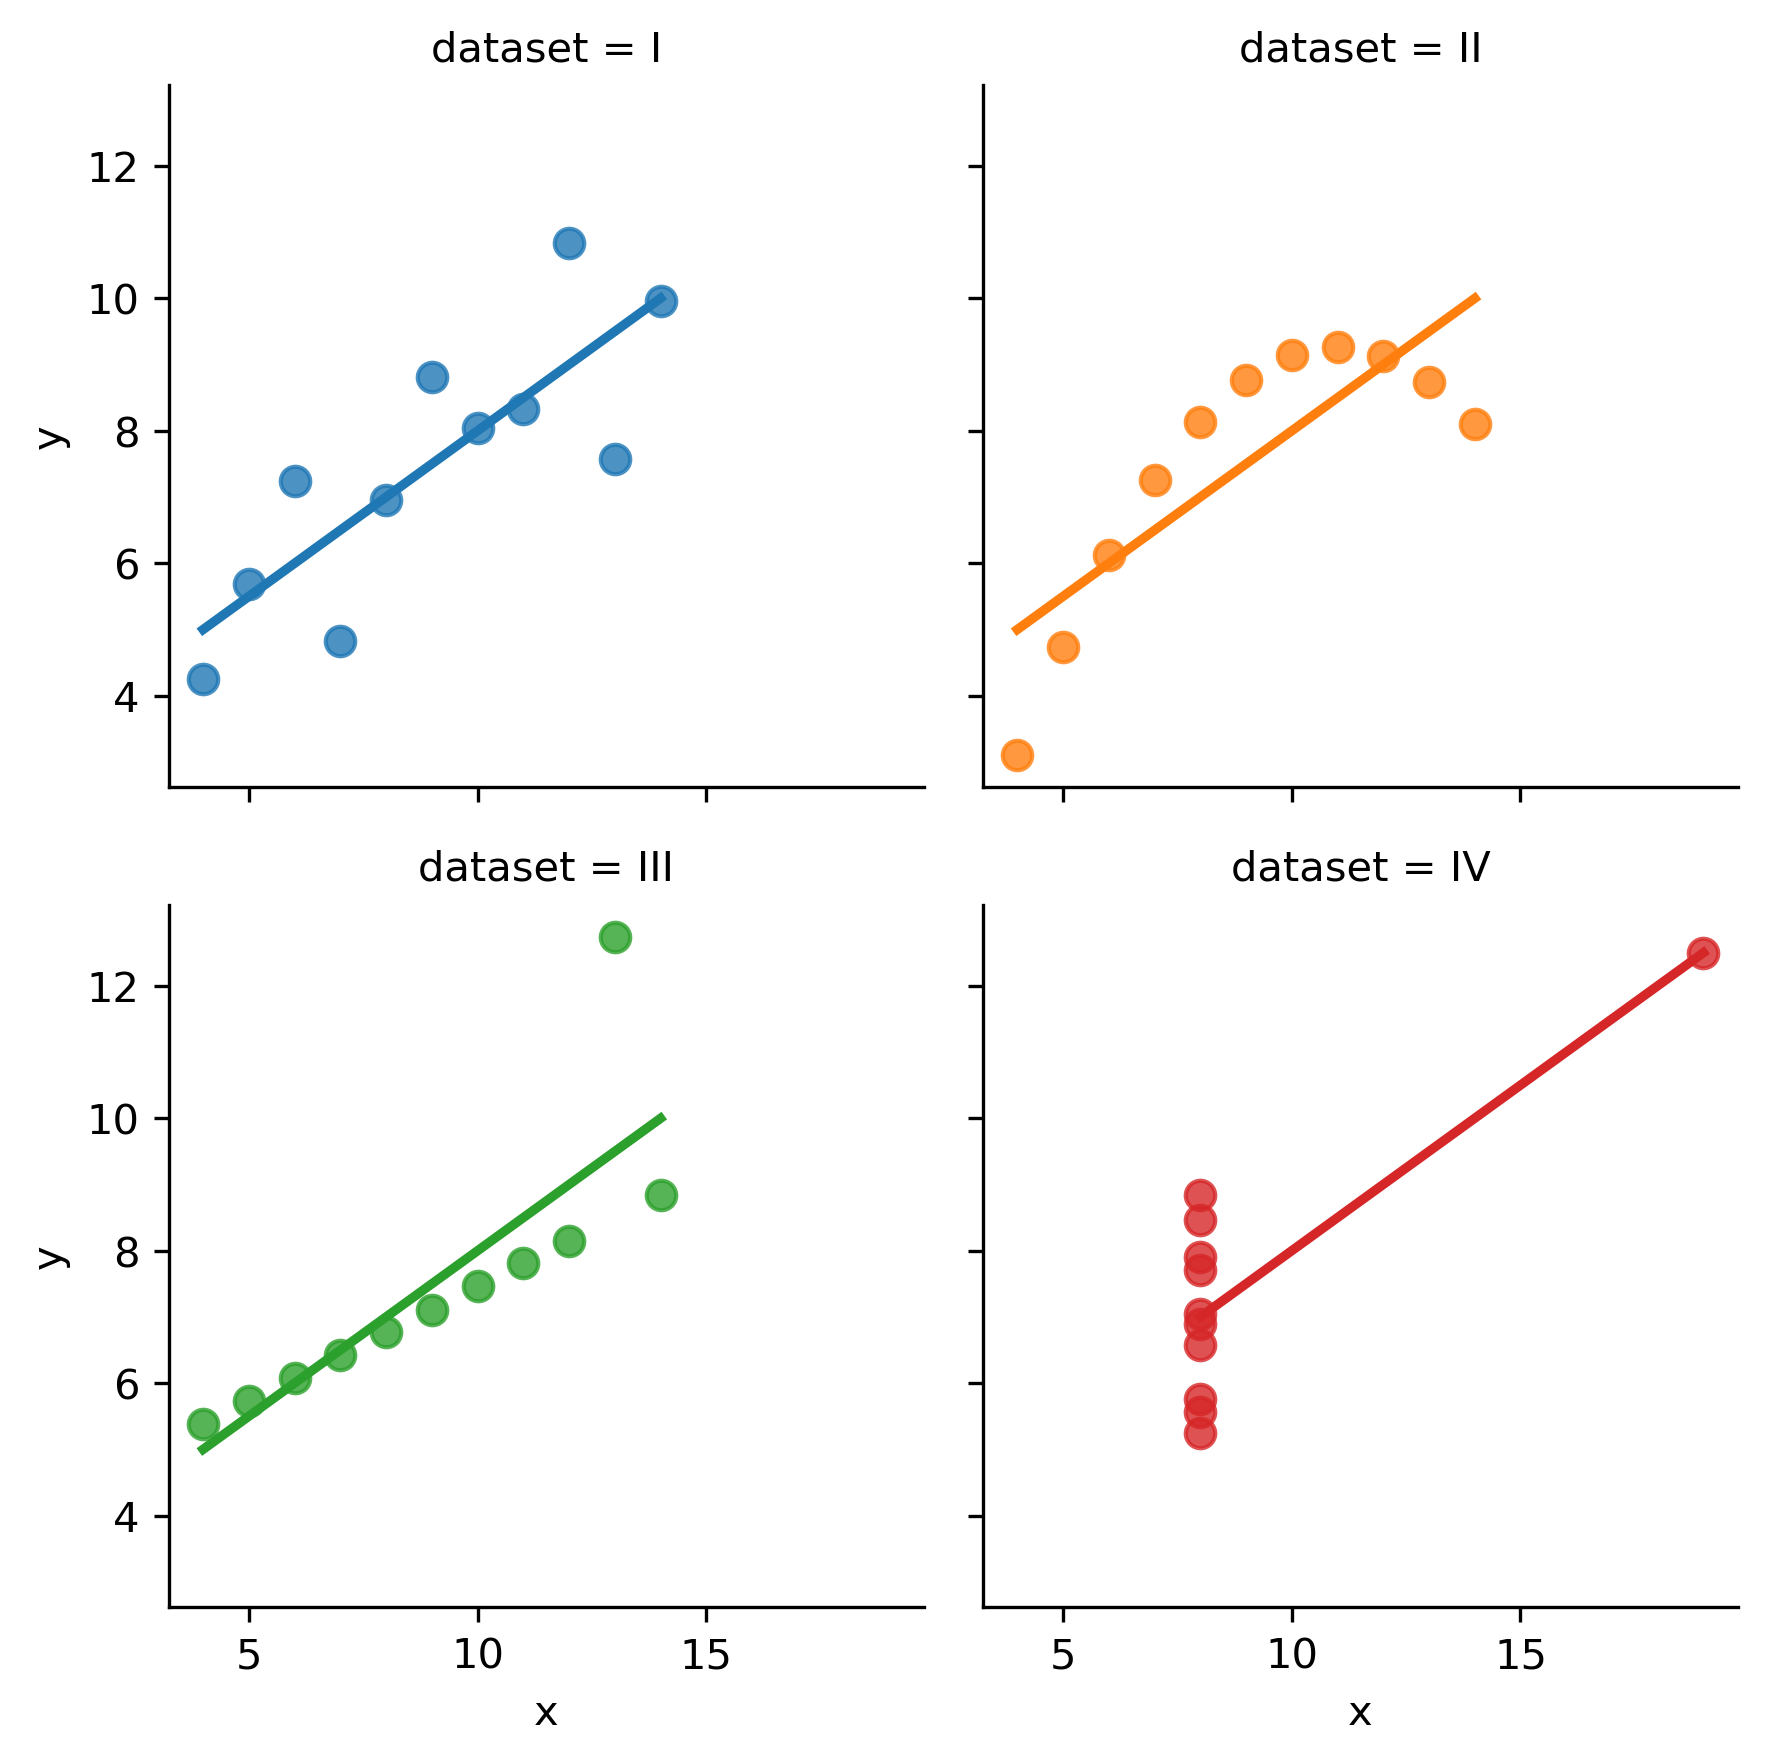
\includegraphics[width=\textwidth]{anscombe_grid.png}}
\caption{Baseline NumPy validation of Anscombe's Quartet, plotted from \texttt{anscombe\_clean.csv}. The visual plots confirm drastically different spatial distributions (linear, non-linear, outlier-driven) despite sharing the exact same calculated regression trajectories.}
\label{fig:anscombe}
\end{figure}

\newpage
\section{Methodology Phase III: Datasaurus Dozen Scale Validation}
\subsection{Operational Overview and Source Data}
Building upon the Anscombe validation, the third phase scaled the computational architecture to handle complex geometric clustering. Executed via \texttt{03\_datasaurus\_stats\_processing.ipynb}, this phase ingested \texttt{datasaurus\_clean.csv}. This dataset, conceptualized by Matejka and Fitzmaurice \cite{matejka2017}, expands the Anscombe illusion to 13 highly distinct spatial shapes. 

\subsection{Baseline Metric Extraction}
The dataset was logically partitioned using Pandas \texttt{groupby} operations. The custom NumPy engine was iterated over each subset to extract the immutable baseline metrics that would later serve as the constraints for the optimization phase. 

By applying the logic to the primary \textit{dino} subset, the pipeline locked in the following constants:
\begin{itemize}
    \item \textbf{Mean:} $X = 54.2633$, $Y = 47.8323$
    \item \textbf{Variance:} $X = 281.0700$, $Y = 725.5160$
    \item \textbf{Pearson Correlation:} $-0.0645$
    \item \textbf{OLS Regression:} $y = 53.45 - 0.10x$
\end{itemize}

\begin{figure}[H]
\centerline{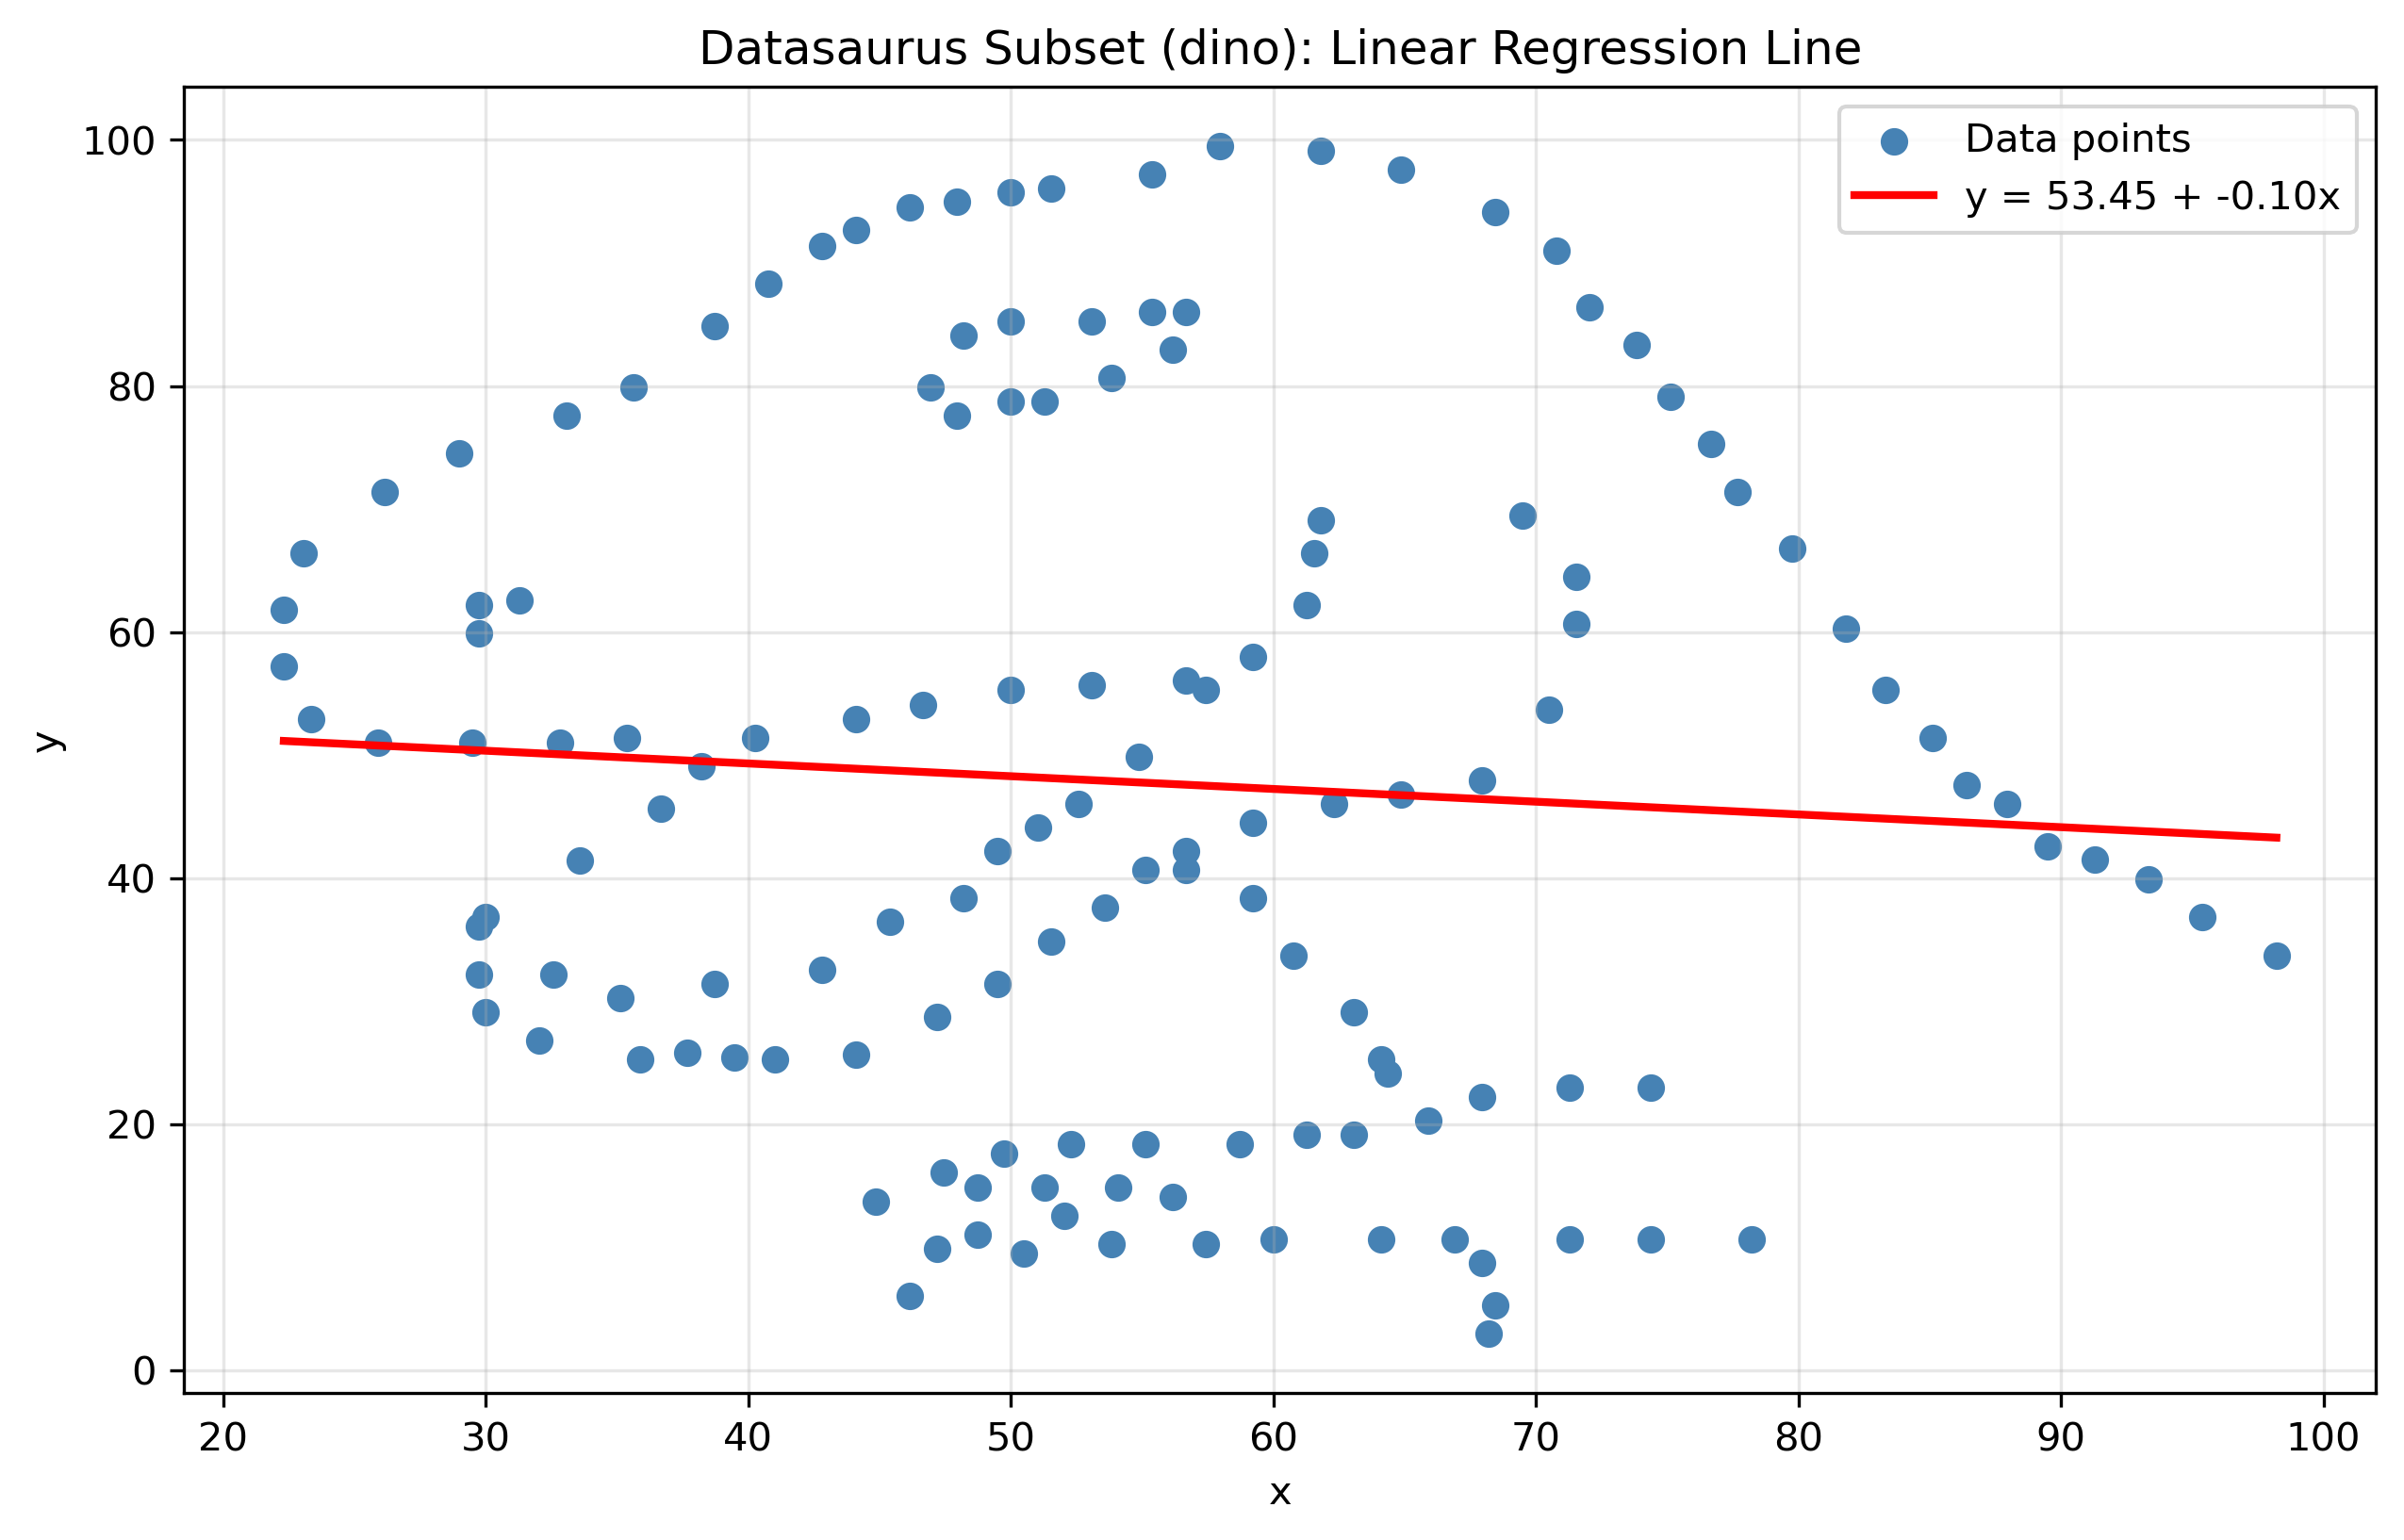
\includegraphics[width=0.8\textwidth]{dino.png}}
\caption{The unperturbed baseline Datasaurus geometry alongside its least-squares regression line, establishing the starting physical state for the final morphological engine.}
\label{fig:dino}
\end{figure}

\subsection{Scale Validation Results}
The operation confirmed that despite forming completely different geometries—including concentric circles, a five-pointed star, and a dinosaur—all 13 datasets return the exact same baseline statistics. This phase definitively proved that relying on summary statistics without high-resolution visual rendering can mask extreme spatial variances in data science pipelines.

\begin{figure}[H]
\centerline{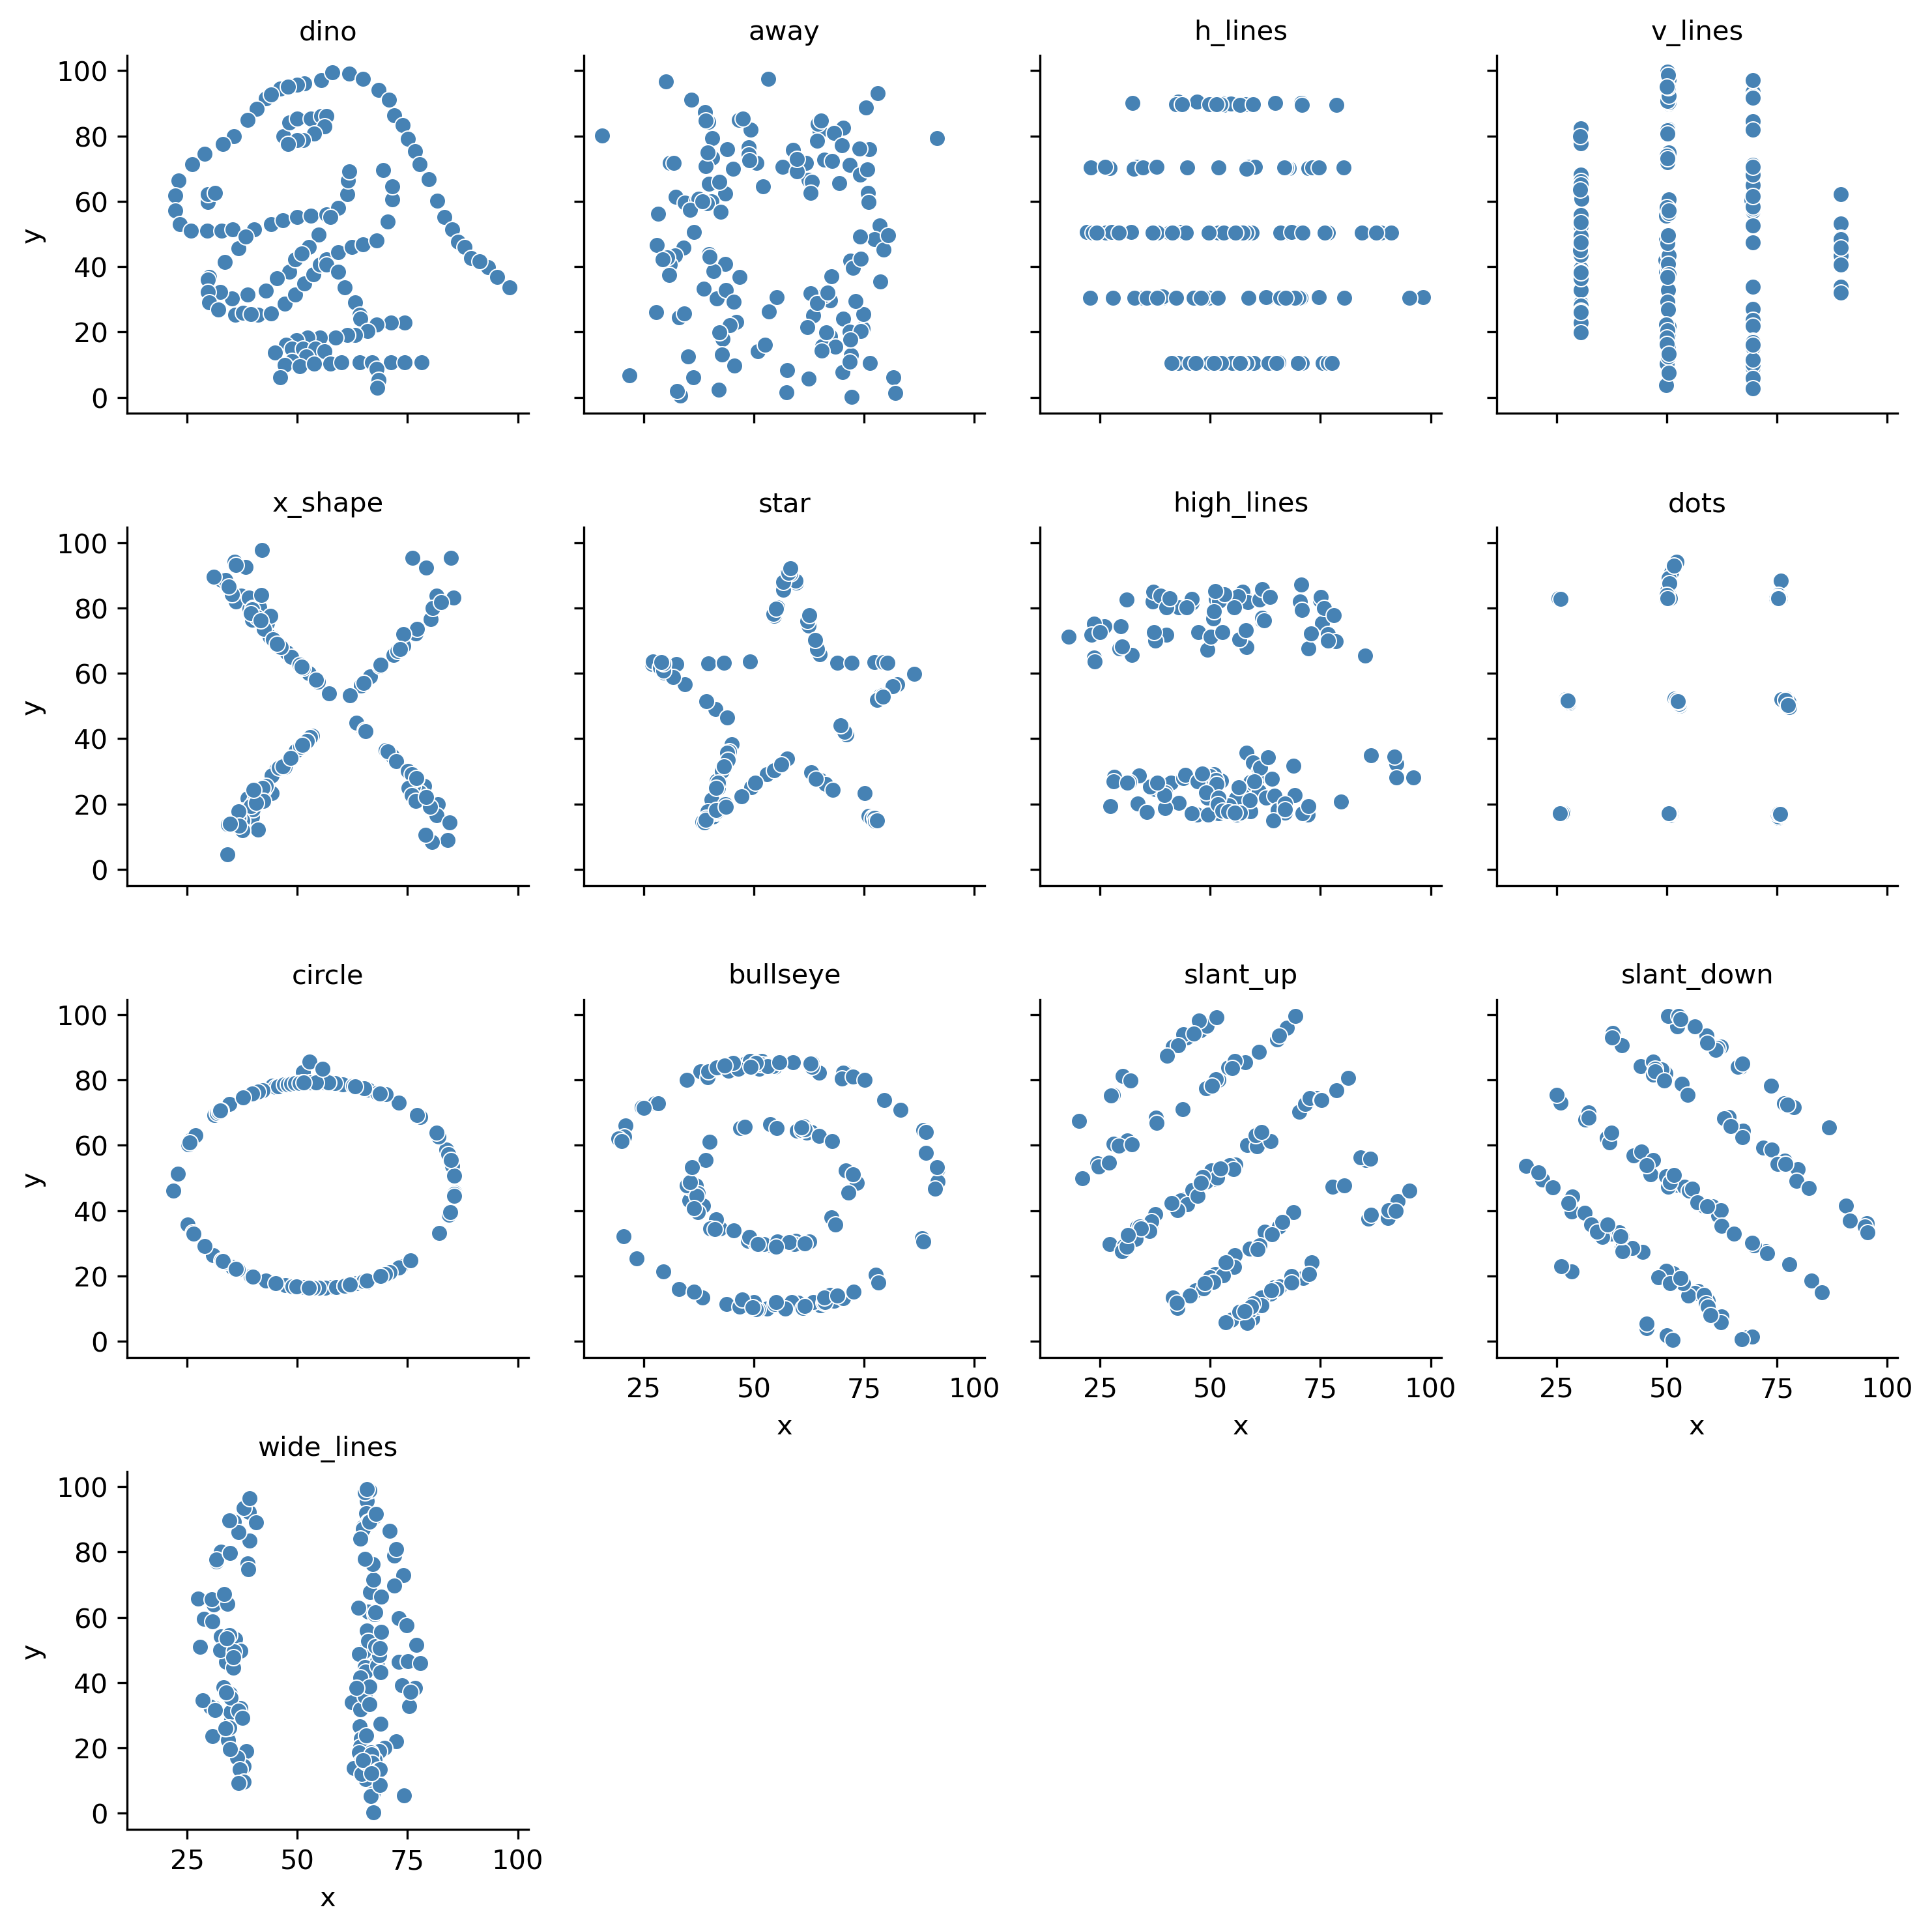
\includegraphics[width=\textwidth]{datasaurus_grid.png}}
\caption{Visual representation of the Datasaurus Dozen subsets. Computed via the custom NumPy engine, every shape pictured shares identical mean, variance, Pearson correlation coefficients, and least-squares regression lines.}
\label{fig:datasaurus_grid}
\end{figure}

\newpage
\section{Methodology Phase IV: Simulated Annealing Optimization Engine}
\subsection{Operational Overview and Source Data}
The final phase operationalized the theoretical framework of Matejka and Fitzmaurice \cite{matejka2017} by deploying a stochastic optimization engine. Executed within \texttt{04\_simulated\_annealing.ipynb}, the engine ingested the \textit{dino} subset from \texttt{datasaurus\_clean.csv} with the objective of morphing its coordinates into the \textit{star} geometry without violating the established statistical baseline.

\subsection{The Statistical Gatekeeper}
The optimization algorithm was engineered with a strict mathematical Gatekeeper. During each iteration, a spatial coordinate was randomly selected and perturbed utilizing Gaussian noise:
\begin{equation}
x_{new} = x_{old} + \mathcal{N}(0, \sigma^2), \quad y_{new} = y_{old} + \mathcal{N}(0, \sigma^2)
\end{equation}

Immediately following the perturbation, the entire coordinate array was re-evaluated through the NumPy engine. If the new perturbation shifted the mean, variance, Pearson correlation, or least-squares trajectory away from the baseline by a margin greater than $0.1$, the move was universally rejected. This ensured the statistical signature remained physically immutable.

\subsection{Thermodynamic Optimization and Acceptance Probability}
If the Gatekeeper accepted the perturbation, the algorithm calculated the new spatial cost, defined as the Euclidean distance between the perturbed point cloud and the target \textit{star} geometry. 

Moves that decreased the spatial cost were automatically accepted. However, to prevent the point cloud from clustering into suboptimal local minima, moves that \textit{increased} the spatial cost were accepted probabilistically based on the principles of thermodynamics. The acceptance probability was governed by the system temperature $T$:
\begin{equation}
P(\text{Accept}) = \exp\left(\frac{-\Delta \text{Cost}}{T}\right)
\end{equation}
The engine was initialized with a temperature of $T = 100.0$ and subjected to an exponential cooling decay rate of $0.9995$ over 150,000 algorithmic iterations.

\newpage
\section{Final Results and Conclusion}
The initial spatial divergence between the \textit{dino} configuration and the \textit{star} configuration was calculated at a Euclidean cost of $1103.80$. Following the completion of the 150,000 optimization cycles, the final spatial cost plummeted to $216.86$, achieving an $80.35\%$ reduction in spatial error.

\begin{figure}[H]
\centerline{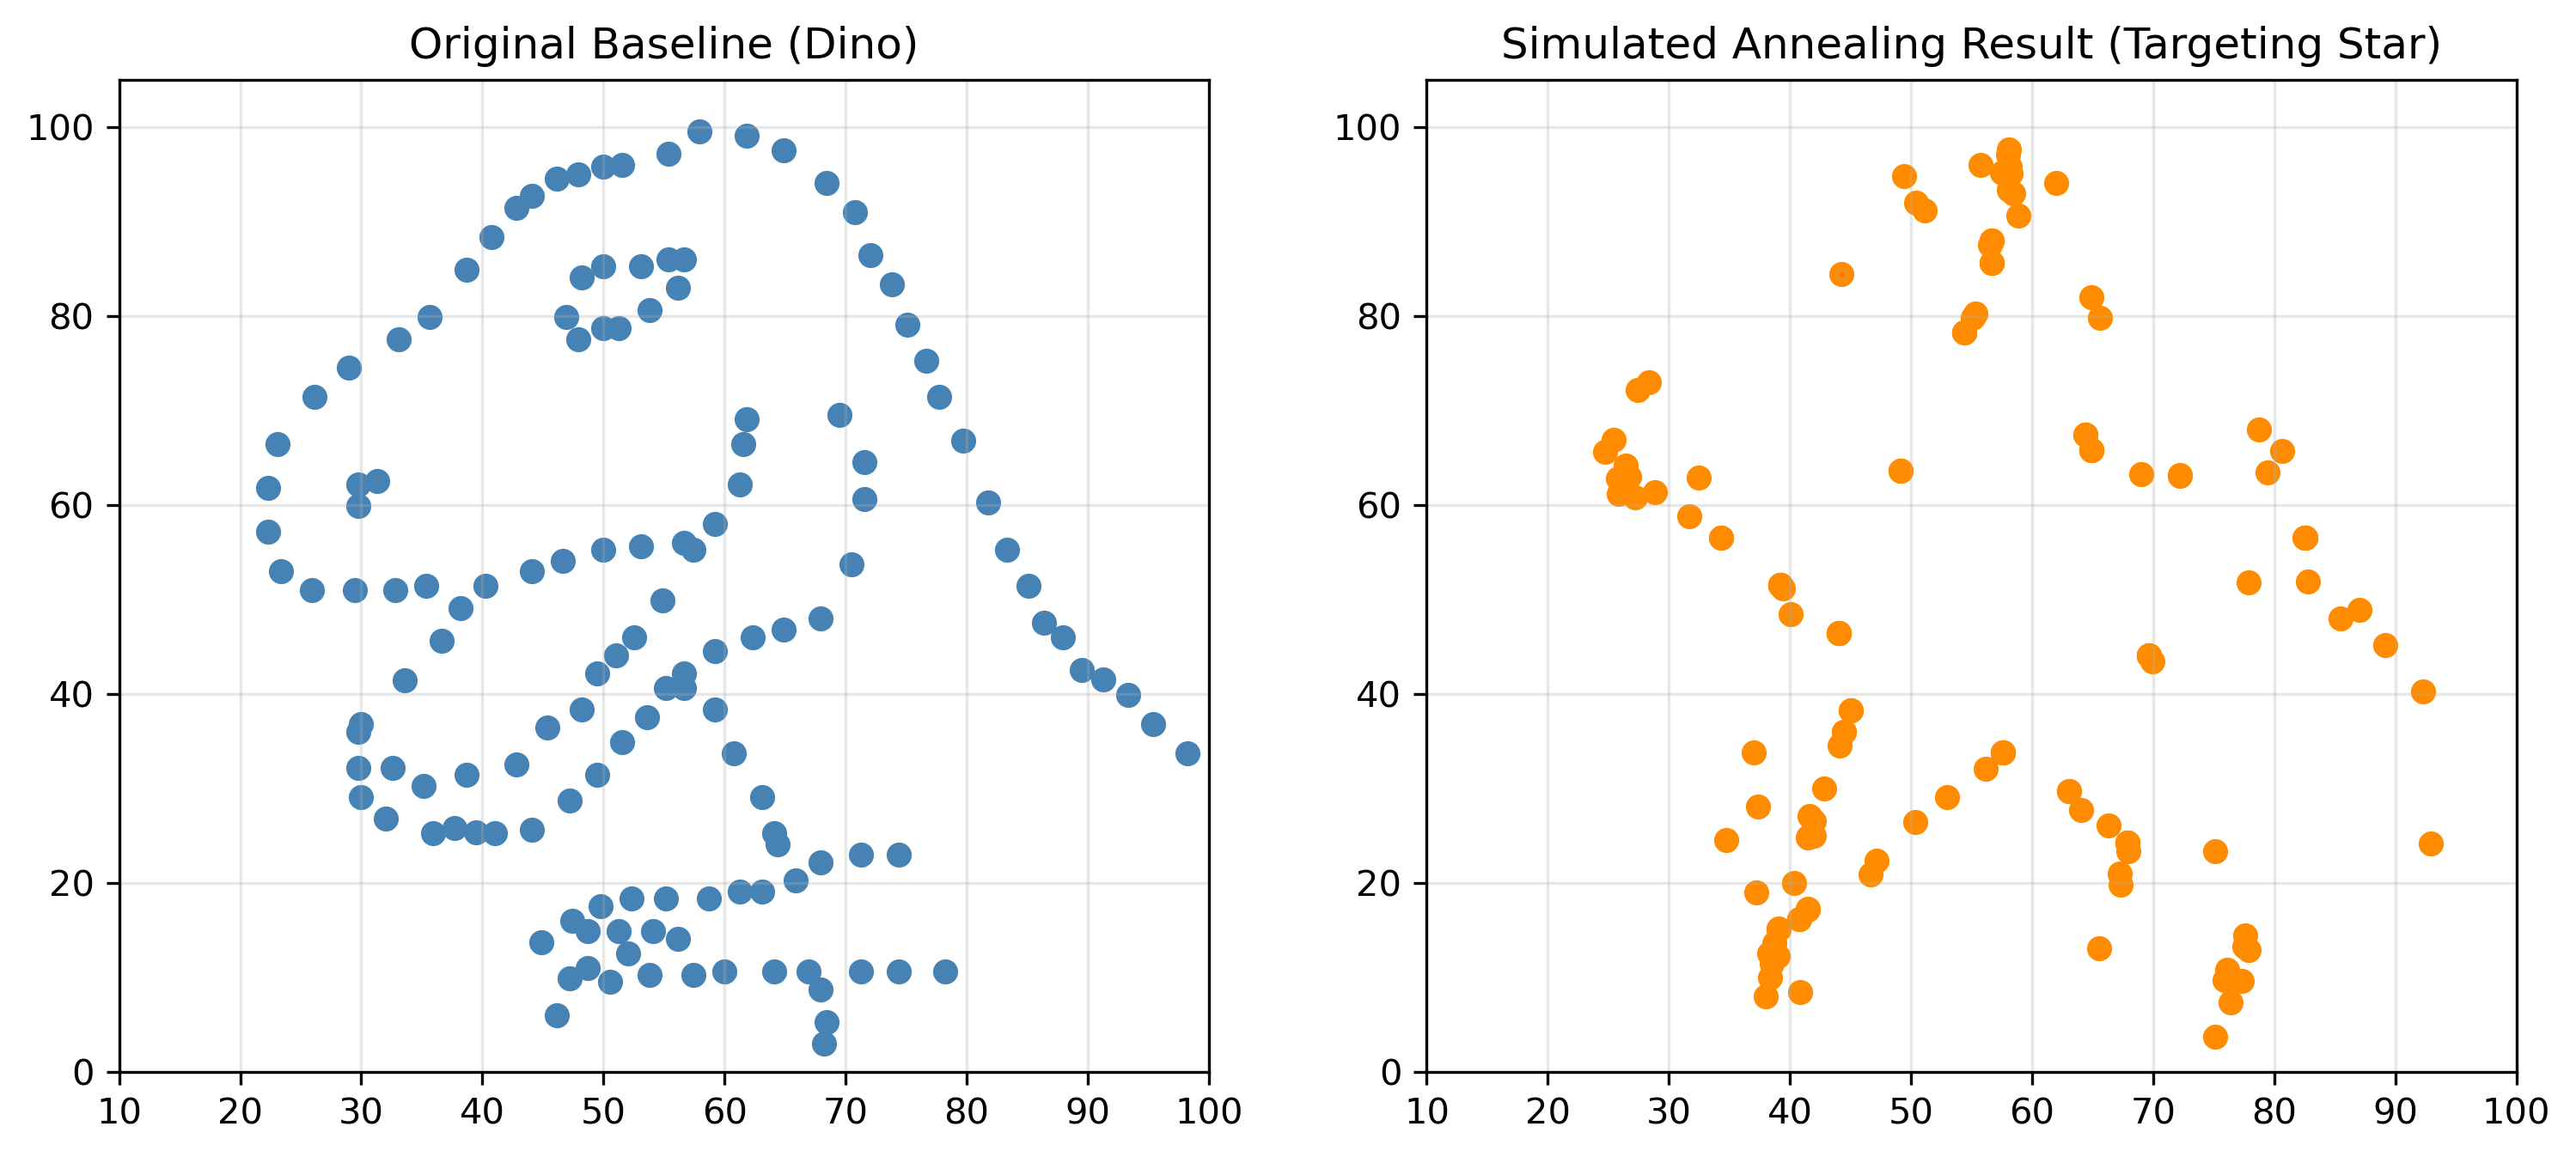
\includegraphics[width=\textwidth]{star_sa.png}}
\caption{Side-by-side comparison of the baseline \textit{dino} geometry and the final morphological output targeting the \textit{star} geometry. Both visual structures possess mathematically identical statistical signatures.}
\label{fig:star_sa}
\end{figure}

The optimization successfully reorganized the point cloud into the target star shape (Figure \ref{fig:star_sa}). The slight geometric noise observed in the final plot is the direct physical manifestation of the $0.1$ tolerance Gatekeeper. The Simulated Annealing engine discovered the absolute closest spatial approximation of a star that mathematically still functions as a dinosaur. 

Ultimately, this implementation proved that summary statistics are a mathematically incomplete metric for evaluating data distributions. The successful deployment of the Simulated Annealing engine demonstrates that data can be deliberately manipulated into highly specific spatial configurations without ever triggering baseline statistical alarms, highlighting the mandatory requirement for exploratory spatial visualization.

\newpage
\begin{thebibliography}{9}
\bibitem{anscombe1973} 
Anscombe, F. J. (1973). 
\textit{Graphs in Statistical Analysis}. 
The American Statistician, 27(1), 17-21.

\bibitem{matejka2017} 
Matejka, J., \& Fitzmaurice, G. (2017). 
\textit{Same Stats, Different Graphs: Generating Datasets with Varied Appearance and Identical Statistics through Simulated Annealing}. 
Proceedings of the 2017 CHI Conference on Human Factors in Computing Systems (pp. 1290-1294).
\end{thebibliography}

\end{document}